\subsection{Prospectively frozen closed-loop instruction necessity}
\label{sec:instruction-necessity}

High task success alone does not show that a policy uses its instruction. Before these outcomes
were observed, we fixed a paired test on canonical episodes $40$--$49$ for every task and the
same three checkpoints. Each checkpoint-state pair was rolled out for the full $280$-step horizon
under the correct familiar instruction, one deterministic outcome-independent co-present control
instruction, and an empty instruction. All conditions shared the exact initial physical input and
their order was chosen by a frozen hash. Co-presence was verified from simulator observation
fields and does not guarantee unoccluded camera visibility. The empty string encodes tokenizer
BOS plus $31$ unmasked PAD tokens, together with the model's learned common BOS.

\begin{figure}[H]
\centering
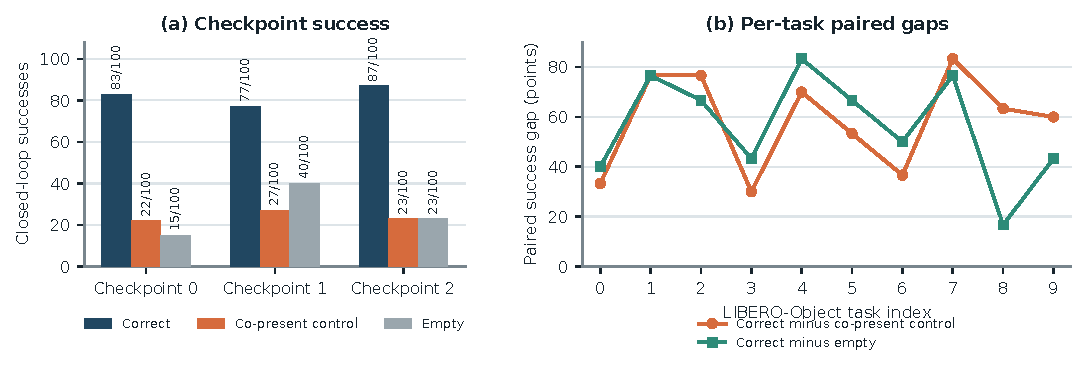
\includegraphics[width=0.98\textwidth]{../paper_figures/instruction_necessity_closed_loop.pdf}
\caption{\textbf{Closed-loop instruction necessity on familiar tasks.} Left: exact successes
among $100$ paired canonical states per checkpoint. Right: correct-instruction success minus each
control, pooling the three checkpoint outcomes for each task. All ten task gaps are positive for
both controls at the task-aggregate level.}
\label{fig:instruction-necessity}
\end{figure}

Across $100$ unique canonical states and three checkpoints, the correct instruction succeeds on
$247/300=82.3\%$ of checkpoint-state pairs. The co-present control succeeds on $72/300=24.0\%$
and the empty instruction on $78/300=26.0\%$, giving paired gaps of $58.3$ and $56.3$ points.
Correct-instruction success is $83/100$, $77/100$, and $87/100$ by checkpoint, and both paired
gaps are positive for every checkpoint aggregate. All ten pooled task aggregates are strictly
positive for both controls. One-sided exact McNemar tests give $p=2.02\times10^{-45}$ and
$p=1.52\times10^{-44}$. These pooled tests use $300$ checkpoint-state pairs and are not
cluster-robust inference. A frozen $20{,}000$-draw task-stratified state-cluster bootstrap
resamples $100$ unique task-episode states while retaining all three checkpoint outcomes. Its
$95\%$ intervals are $[51.0,65.7]$ and $[50.0,62.3]$ points. Every prospectively frozen gate
passes.

This establishes instruction necessity for familiar LIBERO-Object prompts, objects, scenes,
tasks, and checkpoints. Appendix~\ref{app:instruction-embedding-ablation} gives a disjoint paired
test that isolates the learned lexical-embedding path. Neither test establishes counterfactual
goal following, paraphrase robustness, unseen-object or compositional grounding, cross-suite or
physical transfer, or a benefit unique to tensor decomposability.
